\documentclass[12pt]{article}
% $Id: bioperl-article.tex,v 1.31 2002-04-22 17:14:53 jason Exp $
% $Log: not supported by cvs2svn $
% Revision 1.30  2002/04/22 17:02:57  jason
% changes to let figure2 be submitted separately and include a little more clarity in discussion
%
% Revision 1.29  2002/04/19 03:56:04  lapp
% Mostly typographical corrections. Some little polishing of the discussion
% section about others' failures.
%
% Revision 1.28  2002/04/16 20:36:10  jason
% remove personal communication
%
% Revision 1.27  2002/04/16 20:32:11  jason
% added figure 2 back in and simplified caption, also fixed a couple of typos and a added some flow to the discussion
%
% Revision 1.26  2002/04/16 15:06:38  jason
% rough changes to discussion -- need a rework
%
% Revision 1.25  2002/04/12 18:39:38  lstein
% Edits following conference call between Jason, Lincoln and Hilmar.
%
% Revision 1.24  2002/04/12 05:37:28  lapp
% Corrected a few more typos and errors. Rest for tomorrow's phone
% conference.
%
% Revision 1.23  2002/04/12 03:12:09  jason
% caption text fixes and fixed small bug in the figure 2 code
%
% Revision 1.22  2002/04/11 15:53:05  jason
% small editorial changes and tense correction
%
% Revision 1.21  2002/04/10 03:31:13  jason
% spelling changes, updated title
%
% Revision 1.20  2002/04/09 20:38:30  jason
% Added reference to the figures and Table 1 -- these appear at the end of my PDF document when using pdflatex
%
% Revision 1.19  2002/04/09 19:44:34  lstein
% Minor grammar and typographical fixes from lincoln
%
% Revision 1.18  2002/04/07 20:47:05  jason
% merged in most of Hilmar's comments with some edits.  I think 3 main things are left to polish: Abstract, Conclusion, and Interoperability
%
% Revision 1.17  2002/04/07 08:30:41  heikki
% minor fixes
%
% Revision 1.16  2002/04/06 19:07:08  lapp
% Spelled out GNF.
%
% Revision 1.15  2002/04/05 23:15:32  jason
% some changes to format towards GR - a few sentance reworks and transitions - cut it down to 5 main topics, pages for weblinks and each figure with captions
%
% Revision 1.14  2002/04/05 17:19:02  jason
% grammatical changes
%
% Revision 1.13  2002/04/02 00:07:13  jason
% rework, with Mark's comments - still need to add Matt's suggestions
%
% Revision 1.12  2002/03/25 14:17:28  jason
% small TeX bugs
%
% Revision 1.11  2002/03/24 20:49:13  jason
% reworking abstract, removed redundancy and greatly simplified the interoperability section.  Need to condense to probably 4-5 main sections
%
% Revision 1.10  2002/03/21 21:50:04  jason
% reworked abstract for GR and moved examples around.  Reworked abstract for GR and moved examples around.  Added statistics about tests and number of modulesTable for Modules rather than list.
%
% Revision 1.9  2002/03/19 10:58:47  heikki
% fixing examples, lot's of typos in the docs, minor changes
%
% Revision 1.8  2002/03/13 21:21:08  jason
% 3rd draft - with Lincoln's changes
%
% Revision 1.7  2002/03/04 22:18:09  jason
% Some reworking of text, placeholders for expansion on the major 
% theme of open-source developmentmore references and testing out 
% the lstlisting for code section, lines
% are not wrapping nicely though in 2-column mode with the code,
% Author list still incomplete and need to move acknowledgements
% around some more
%

\usepackage {listings,hyperref,url,apalike,layouts,
	     	pstricks, epsfig,graphicx,keyval,fancyhdr,
	     setspace,fullpage }

\begin{document}

\doublespacing

\title{The Bioperl Toolkit: Perl modules for the life sciences}
\author{Jason E Stajich$^1$$^*$ \and Hilmar Lapp$^2$ \and Heikki Lehv\"{a}slaiho$^3$ \and Lincoln D Stein$^4$ \and Ewan Birney$^3$ \\
$^1$ \small{\textit{University Program in Genetics, Duke University,
Durham, NC 27710 USA}} \\
$^2$ \small{\textit{Genomics Institute of the Novartis Research
Foundation (GNF), San Diego, CA 92121 USA}} \\
$^3$ \small{\textit{European Bioinformatics Institute, Welcome Trust
Genome Campus, Hinxton, Cambridge CB10 1SD, UK}} \\
$^4$ \small{\textit{Cold Spring Harbor Laboratory, Cold Spring Harbor, NY 11724 USA}}\\
}
\maketitle
\begin{abstract}

The Bioperl project is an international open source collaboration of
biologists, bioinformaticians, and computer scientists that has
evolved over the last 7 years into the most comprehensive library of
Perl modules available for managing and manipulating life science
information.  Bioperl provides an easy-to-use, stable, and consistent
programming interface for bioinformatics application programmers.  The
Bioperl modules have been successfully and repeatedly used to reduce
otherwise complex tasks with only a few lines of code.  The Bioperl
object model has been proven to be flexible enough to support
enterprise-level applications such as EnsEMBL while maintaining an
easy learning curve for novice Perl programmers.  Bioperl is capable
of executing analyses and processing results from programs such as
BLAST, ClustalW, or the EMBOSS suite.  Interoperation with modules
written in Python and Java is supported through the evolving BioCORBA
bridge.  Furthermore, Bioperl provides access to a common sequence
data storage by fully supporting the standards of the Open
Bioinformatics Database Access project.  This paper describes the
overall architecture of the toolkit, the problem domains which it
addresses, and gives specific examples of how the toolkit can be used
to solve common life sciences problems.  We conclude with a discussion
of how the open source nature of the project has contributed to the
development effort.

Bioperl is available as open source software free of charge and
licensed under the Perl artistic license at \url{http://www.bioperl.org/}.  
Support inquiries should be addressed to \url{bioperl-l@bioperl.org}.

\textbf{Keywords:} Bioinformatics Software Perl

$^*$To whom correspondence should be addressed.

\end{abstract}

\section{Introduction}

Computational analysis is an integral part of modern biological
research.  Numerous computer software tools exist to perform data
analyses, but it is not simple to automatically combine data and
results from multiple sources without the use of computer software
designed to read and write data specific to the biological domain.
The day-to-day work in a typical bioinformatics lab consists largely
of writing program logic to achieve this data integration.

One programming language, Perl, is one of the most widely used
programming languages for these tasks, and is commonly thought of as
the language most easily grasped by newcomers to the field.  Perl has
been extremely successful for connecting software applications together into
sequence analysis pipelines, converting file formats, and extracting
information from the output of analysis programs and other text files.

Much of the Perl software in bioinformatics is specific to a
particular lab or institution and is written for immediate
utility, not reusability.  The Bioperl toolkit brings together
reusable Perl modules containing generalized routines specific to life
science information.  A primary motivation behind writing the toolkit
is the authors' desire to focus energies on a solution whose
components can be shared rather than duplicating effort.  In our
minds, once a routine is written for parsing and interpreting sequence
from EMBL and Genbank format sequence files, no one else should have
to worry about writing their own.  In this spirit we chose to make our
code freely available under an open source license
\cite{open-source-ref} so that others could contribute their solutions
to the project as well.  Just as the Human Genome Project was speeded
and made more efficient by public sharing of data, so has the open
nature of the Bioperl project reduced the time for solutions and new
tools to reach the community \cite{waterston}.

However, to be adopted by the community our software has to be user
friendly.  To that end we have provided extensive documentation
of all the methods in each module, a graphical diagram of the objects
in the toolkit, and tutorials with simple solutions to common tasks.
Additionally we have created a module which provides
simplified functions, such as \textit{read\_sequence} to read
in sequences from a file, to provide entry-level access to the toolkit.
The goal of Bioperl is to help a user focus
on her specific problem at hand, such as the logic needed to filter
hits in a BLAST \cite{blast} report by certain criteria, rather than
on the actual mechanics of \textit{parsing} that BLAST report.

\section{Methods}

The Bioperl project began in 1995 \cite{chervitz-bits} at a time when
there were few programming toolkits for manipulating biological data
or results from sequence analysis programs.  Although Perl had already
gained widespread popularity in the bioinformatics community for its
efficient support of text processing and pattern matching tasks, there
were in fact no biological toolkits available in this language.

The project grew out of the following observations.  
\begin{itemize}

\item First, even though file formats of different analysis programs
are different, the information they represent is the same.  For
example, a pair-wise alignment is always between two sequences and has
common properties such as length, score, fraction of identities, start
and end of the aligned sequences, and so forth.

\item Second, the number of data structures needed to represent
information flow is limited, and common to most applications, such as
sequences, annotation, features, and alignments.  This permits a 
small set of modules to be reused for a variety of purposes.

\item Third, a set of operations is commonly performed on these data
structures.  These include reading and writing information to a file,
querying a sequence for its features, and translating a coding
sequence into protein.

\end{itemize}

This scenario naturally lends itself to the principle of
object-oriented programming, which Perl emulates with modules.

Object-oriented programming is the practice of grouping related tasks
together into logical and broadly applicable components.  For example,
a DNA Sequence component could contain methods to retrieve the
sequence's accession number, reverse complement the DNA, or translate
it into a protein sequence.

The mission of Bioperl is to provide an easy-to-use object-oriented
Perl library that contains data structures and operations commonly
used in the life sciences as clean, generic, and re-usable modules.
By separating the components into logical groups, such as sequences,
alignments, and databases, we have been able to add features to a
specific module without necessarily affecting the rest of the toolkit
library.  This separation is a key aspect of object-oriented
programming and permits us to produce generic components with a stable
interface for the programmer (the so-called API).  

At present the components and operations in Bioperl center around
biological sequence analysis and annotation.  In the last year the
project has expanded to address new areas including phylogenetics,
maps, protein structure, and bibliographic references.  The project
has over 300 modules and comprises more than 160,000 lines of code and
embedded documentation.  The Perl modules, illustrated in Table
\ref{tab:modules}, are organized by logical names so that, for example,
the Bio::Search hierarchy contains modules related to database
searches and Bio::Graphics contains modules that are related to
drawing (Figure 1).  The Bio::Perl module itself
is a simplified API that provides access to the most-commonly used 
Bioperl functions.

When designing Bioperl objects we sought to provide a
programming interface that is very easy to use but that at the same
time could be easily extended in its capabilities and behavior through
code reuse.  Using an object-oriented paradigm we followed certain
design principles.

\begin{itemize}

\item Separate the interface from the implementation.  The key
information about a component is the method names and their list
of accepted arguments.  Similar in concept to interfaces in Java, we
built interfaces as collections of methods which describe the expected
behavior of a module, but do not do any of the work.  Child classes
implement the interfaces, providing specializations of their parents
to perform specific tasks.  To help distinguish implementation classes from
interface definitions we used a capital 'I' appended to the object
name.

For example, Bio::SeqFeatureI describes the `contract' for all classes
which are sequence features.  For Features this includes methods for
start, end, strand, and access to the annotation table via tag/value
pairs.  All modules in the Bio::SeqFeature hierarchy implement this
interface (Figure 2).  The power of this design is that operations
which expect a Bio::SeqFeatureI, such as operations in the
Bio::Graphics modules, can operate on anything which implements the
Bio::SeqFeatureI interface.  In this manner, sequence annotation that
is retrieved from a DAS server \cite{das}, a local file, or a database
server can all be drawn as an image with the same methods in the
Bio::Graphics modules.

\item Generalize common routines into a single module providing a base
framework for the respective operations.  As an example we centralized
the basic Input/Output (IO) operations into an IO object, called
Bio::Root::IO.  Because all modules that need IO data access use
operations from the IO module, these operations are implemented across
the entire package in a consistent way.  This design choice also
provides a single location for applying improvements to the shared
methods.

\item Employ the Factory and Strategy patterns \cite{gangoffour} as
much as possible. A strategy pattern defines one or more operations a
particular implementation must support. As an example, Bio::SeqIO
defines that implementations support the operation
\textit{next\_seq()}, returning the next sequence in the stream as a
Bio::PrimarySeqI compliant object. Various parsers for the different
sequence formats implement this method, thereby providing one
consistent interface to sequence streams irregardless of the
format. At the same time, Bio::SeqIO acts as a factory by
instantiating the parser appropriate for a particular format without
the caller having to know which module is capable of parsing the
desired format. We implemented the same concept for databank search
result parsers in Bio::SearchIO. The Bio::Factory hierarchy contains
other factories, which can instantiate classes implementing a
particular contract for a desired specialization.

\end{itemize}

Bioperl is written purely in Perl and requires at least version 5.005
of the Perl interpreter (the current stable version of Perl as of the
time of writing is 5.6.1).  The toolkit has been validated for
cross-platform compatibility on most UNIX and UNIX-like operating
systems.  In addition, Bioperl has been tested and runs on Macintosh
OS X and Microsoft Windows operating systems.  

Since the Bioperl toolkit depends on the Perl interpreter, there are a
rare number of cases where its behavior is not consistent across
different versions of Perl or between versions of Perl on certain
operating systems.  Descriptions of these version-specific problems
and their solutions are available from the Bioperl website.

In addition to pure Perl solutions to bioinformatics problems, Bioperl
can take advantage of external data analysis packages.  Bioperl is
capable of parsing the output from a variety of programs including BLAST (both
NCBI and WUBLAST \cite{wublast} versions), HMMer \cite{hmmer}, 
ClustalW \cite{clustalw}, T-Coffee \cite{tcoffee}, 
Phylip \cite{phylip}, many EMBOSS \cite{emboss} programs, 
Genscan \cite{genscan}, and 18 others.
In addition, it can launch remote analyses using the EMBOSS
suite, NCBI BLAST, and the multiple sequence alignment
programs ClustalW and T-Coffee.  In
some cases, when an external package is not available, Bioperl will
fall back to using a slower method, either by emulating the package in
pure Perl or by invoking a network-based analysis service such as the
NCBI BLAST analysis queue.  Additional work is in progress to
incorporate into the project access to remote analysis services at the
European Bioinformatics Institute (EBI) (\url{http://www.ebi.ac.uk}) and
Pasteur Institute (\url{http://www.pasteur.fr}).

In order for us to produce uniform software code, we established
coding guidelines that are extensions of widely accepted
object-oriented programming style.  All modules were required to meet
minimal standards before release.  These standards include a complete
set of regression tests, well formed embedded documentation for each
method, and a concise example code in the SYNOPSIS section of each
module's documentation.  We use the Perl embedded documentation format
(called POD, or Plain Old Documentation) to interleave documentation and
the source code.  This documentation can be converted to text, TeX, or
HTML.  We have used the Pdoc (\url{http://pdoc.sourceforge.net}) tool to
generate colored and hyperlinked documentation in HTML for easy
online browsing.

The development process involves integrated and comprehensive
unit-testing of the code.  We accomplished this by ensuring that each
module has a test in the Bioperl test system.  This style is part of
the Extreme Programming methodology \cite{xprogramming} which we have
adopted in part.  Bioperl 1.0 has over 3000 such tests which the toolkit
passed before release.

To support multiple developers in different time zones and
institutions, the entire Bioperl source code is hosted by the Open
Bioinformatics Foundation (OBF) (\url{http://www.open-bio.org}) on a
CVS server.  CVS, or Concurrent Version Control system
(\url{http://www.cvshome.org}) \cite{cvsbook}, allows multiple
developers to make changes to the software source code concurrently
without having to coordinate every single change.  The ability to
share code easily and quickly has shown itself to be key for
establishing a successful open source project.  OBF also hosts the
Bioperl website at \url{http://www.bioperl.org}.

\section{Results}

Bioperl has 10 active developers led by a core of 5 primary developers
who ensure that standards are met, prepare code releases, and set the
vision for the project.  At the time of publication the mailing lists
for the project include 1300 subscribers and an average of 10,000
unique visitors to our website each month.  The project has been used
in a variety of endeavors including genome sequencing, annotation,
sequence variation elucidation, disease gene discovery, and
comparative genomics.  An example using Bioperl modules to complete
the simple task of retrieving sequences from a remote database is
shown in Figure 3, and an example of parsing a BLAST report can be
seen in Figure 4.

By far the most advanced use of the Bioperl toolkit has come through
the EnsEMBL \cite{ensembl-nar} project.  The basic sequence handling,
file format parsing, and sequence features for annotation model have
been used as building blocks for automatically annotating the
\textit{Danio rerio}, \textit{Drosophila melanogastor},
\textit{Takifugu rubripes}, \textit{Homo sapiens}, and \textit{Mus
musculus} genomes (\url{http://www.ensembl.org}).

Additionally the Genquire \cite{genquire} annotation package is built
on top of the Bioperl object model and stores sequence and annotation
data in a relational database.  The interactive sequence rendering
capabilities are partitioned into a specific Bioperl package called
bioperl-gui.

The Generic Model Organism Browser (GMOD) \cite{gmod}, Distributed
Annotation System Perl (DAS) server \cite{das}, and TFBS
\cite{tfbs} all use the Bioperl object model to describe sequences and
Bioperl tools to complete analyses.  The GMOD system is a web
interface to databases of features for a genome project.  The DAS
system provides researchers a means to locally annotate sequences and
publish the annotations to the community via the DAS XML protocol.
TFBS provides a Perl implementation of objects for DNA sequence pattern
representation by matrix profiles, with associated methods for searching
the sequences for the occurrence of patterns, pattern storage, and
generation of new patterns. The implementation uses Bioperl sequence,
alignment, sequence features, and feature pair objects.

\subsection{Interoperability}

Sometimes the best solution for a bioinformatics problem is a hybrid
of multiple tools.  These tools, written in different programming
languages such as C, Java, and Python, can be used within a Perl
script simply by invoking them (a process often called ``shelling
out'').  In some situations these tools require that data be available
in a certain format or within a certain database.  Bioperl provides
software layers which can, for example, populate a database with
sequence information which can be accessed and used to generate an
interactive graphical interface provided by the Biojava toolkit.
In other cases, Bioperl is used to create files in a format recognized
by other programs so that they can perform their analyses. 

Bioperl also supports a number of Extensible Markup Language (XML)
standard data exchange formats accepted in the Bioinformatics
community.  Previous work has outlined scenarios where XML has been
useful in a biological context \cite{xmlbioinformatics}.  XML
standards supported by Bioperl include the sequence markup formats
Bioinformatics Sequence Markup Language (BSML;
\url{http://www.bsml.org}) and Berkeley Drosophila Genome Project's
(\url{http://www.fruitfly.org}) Genome Annotation Markup Elements
(GAME; \url{http://www.bioxml.org/dtds/index.html}), NCBI BLAST XML
for BLAST reports, and the bibliographic standards Medline XML
provided by the European Bioinformatics Institute's Bibliographic
Query Service (BQS; \url{http://industry.ebi.ac.uk/openBQS/}) and
Entrez Pubmed XML format \cite{entrez}.

Software can interoperate with other software not only through the
invocation of external programs, but also through invoking methods on
remote components possibly written in a programming language different
from the calling component.  Such a mechanism constitutes the tightest
integration of re-usable software components in a language-independent
way.  The Common Object Request Broker Architecture (CORBA)
\cite{corba} provides an architecture for enabling this technology.
This technology has been applied to biological data at the EBI in
their Radiation Hybrid \cite{rhdb} and EMBL Nucleotide Databases
\cite{embl-corba}.  CORBA implementations are available from
commercial vendors (e.g., Inprise's VisiBroker, IONA's ORBacus) as
well as from open source projects (e.g. ORBit, MICO).  Bioperl is
compliant with the BioCORBA project (\url{http://www.biocorba.org}),
one of the proposed standards for CORBA components for biological
processes.  BioCORBA is also supported by the Biojava
(\url{http://www.biojava.org}) and Biopython
(\url{http://www.biopython.org}) projects.  The standard is under
consideration for adoption by the Object Management Group's Life
Science Research group (\url{http://lsr.ebi.ac.uk}) and is included in
the proposed Open Bioinformatics Database Access (OBDA;
\url{http://obda.open-bio.org}) standard for sequence data access.

\section{Discussion}

Open source development has proven to be a valuable and productive
mechanism for creation of the toolkit.  No single individual owns the
project, rather it is owned by the community of contributors.  The
community approach prevents the death of a project due to loss of
interest by the sole developer and does not permit project stagnation
in the confines of a single laboratory where a single individual or
group is responsible for the continued vitality of a project.  The
original Bioperl project team has been completely replaced over the
last 7 years as members leave the project and new contributors join,
however the direction and focus of the project has continued to expand.

Throughout the development process we learned a great deal about
appropriate software practices for a diverse group of contributors.
The extreme programming methods, which include defining use cases for
our software, establishing a comprehensive regression test suite, and
utilizing code reviews or audits of contributed source code, helped
the community develop code that is compatible and consistent.  The
principles of good design and good documentation have made it easier
for new developers to join the project.

Any collaborative software projects faces challenges, and
bioinformatics projects face additional challenges because of the complex
problem domain.  Often in bioinformatics, the developers are pursing
their own research and software production is a side project to assist
in a specific task.  Previous collaborative efforts have produced
unsatisfactory results due mostly to lack of commitment to open source
principles for the development.  BioWidgets, an early attempt to
create a toolkit was ultimately unsuccessful because the participants did
not commit to open source policies for the software.  Software was
eventually withdrawn from the project because of intellectual property
disputes (N. Goodman, personal communication).  The NCBI toolkit
(\url{ftp://ftp.ncbi.nih.gov/toolbox/ncbi_tools/}), a powerful and highly functional C-language based
toolkit, does not have the widespread usage that it deserves
because of acknowledged deficiencies in its documentation and a closed
development process.  Bioperl does not suffer from these weaknesses
because it cannot be withdrawn from the public domain and it cannot
become a commercial entity which requires users to pay licensing
fees.

We feel that much of the success of the Bioperl toolkit can be
attributed to the open source nature of the project which has allowed
a diverse group of individuals to participate in a collaborative effort.
We have successfully encouraged users of the toolkit to assist in the
development by contributing bug fixes, documentation enhancements, and
new functionality for the benefit of all users.  Contributors are part
of academic, governmental, non-profit, pharmaceutical, and
commercial bioinformatics groups on every continent.  This collaboration and
the guiding principle to get working products written in an extensible
manner have made Bioperl an excellent platform for Perl bioinformatics
software development.  The open sharing and discussion of ideas that
embodies the scientific spirit has proven to be successful in the
world of scientific software development as well.

In the future, Bioperl will continue to evolve to address more domains
of bioinformatics.  We plan to create objects to manage sequence
assembly information, haplotype maps, gene expression, and protein
interaction data.  Additionally, projects focusing on multi-species
comparisons will build Perl modules to manage alignment and syntenic
information.  We will create software layers to interact with OBDA
databases, develop a generic analysis pipeline system to provide
automated analysis components, and expand the supported file formats
the toolkit can read and write.

\section{Acknowledgments}

In alphabetical order, the Bioperl Core is Ewan Birney, Hilmar Lapp,
Heikki Lehv\"{a}slaiho, Jason Stajich, and Lincoln Stein.  The project
has seen significant contributions from the following people, given in
alphabetical order: David Block, Kris Boulez, Steven Brenner, Brad
Chapman, Steve Chervitz, Michele Clamp, Tony Cox, James Cuff, Chris
Dagdigian, Andrew Dalke, Allen Day, Arne Elofsson, Mark Fiers, Georg
Fuellen, James R Gilbert, Ed Green, Roger Hall, Peter van Heusden,
Joseph Insana, Nicolas Joly, Ian Korf, Aaron J Mackey, Brad Marshall,
Chad Matsalla, Chris Mungall, Emmanuel Mongin, Brian Osborne, Lorenz
Pollak, Matthew Pockock, Todd Richmond, Martin Senger, Peter
Schattner, Elia Stupka, Gert Thijs, Charles Tilford, Andrew Walsh, Kai
Wang, Mark Wilkinson, and Alex Zelensky.

Additional ideas and help came from other OBF project team members
including Jeff Chang, Thomas Down, Keith James, and all of the Bioperl
mailing list members.  Some parts of the object model, especially
locations, were adopted from the excellent work of the Biojava project
and its leaders Thomas Down and Matthew Pocock.

We would like to especially acknowledge Steve Chervitz for his
previous role as Bioperl project leader.  Thanks also to Brian Osborne
and Peter Schattner for their excellent documentation and tutorial
work, and Chris Dagdigian for his tremendous support as system
administrator for the OBF.

The Bioperl project and its sister projects (commonly referred to as
the Bio\{*\} projects) are supported under the umbrella of the Open
Bioinformatics Foundation \url{http://www.open-bio.org}.
OBF is supported by hardware donations from Compaq and Sun
Microsystems, and we graciously accept donated bandwidth and computer
server space from Wyeth.

J.E.S is supported by an NIH Genetics training grant.  Thanks to
F.Dietrich, M.DeLong, M.Hahn for their comments on this manuscript.

\section{References}

\bibliography{bioperl}
\bibliographystyle{apalike} 

\newpage

\section{Website References}
\url{http://industry.ebi.ac.uk/openBQS/}, BQS - Bibliographic Query Service.\\
\url{http://www.bsml.org}, BSML - Bioinformatic Sequence Markup Language. \\
\url{http://www.biocorba.org}, BioCORBA Project. \\
\url{http://www.biojava.org}, Biojava Project. \\
\url{http://www.bioperl.org}, Bioperl Project. \\
\url{http://www.biopython.org}, Biopython Project. \\
\url{http://www.fruitfly.org}, Berkeley Drosophila Genome Project.\\
\url{http://www.bioxml.org/dtds/index.html},  GAME - Genome
Annotation Markup Elements. \\ 
\url{http://www.cvshome.org}, CVS Home Page. \\
\url{http://www.ensembl.org}, EnsEMBL Project Home page. \\
\url{http://www.ebi.ac.uk}, EMBL Outstation - European Bioinformatics
Institute. \\ 
\url{http://www.pasteur.fr}, L'Institut Pasteur (Pasteur Institute). \\
\url{ftp://ftp.ncbi.nih.gov/toolbox/ncbi_tools/}, NCBI Toolkit. \\
\url{http://obda.open-bio.org}, Open Bioinformatics Database Access. \\
\url{http://www.open-bio.org}, Open Bioinformatics Foundation. \\
\url{http://lsr.ebi.ac.uk}, Object Management Group's Life Science Research group. \\
\url{http://opensource.org/docs/definition.html}, Open Source
Initiative - Open Source definition. \\
\url{http://pdoc.sourceforge.net}, Pdoc Home Page. \\
\url{http://forkhead.cgr.ki.se/TFBS/}, TFBS Project. \\

\newpage 

% for right hand top labels

\pagestyle{fancy}
\fancyhf{}
\renewcommand{\headrulewidth}{0pt}

\rhead{Stajich\_Table\ref{tab:modules}}

\begin{table}[h]
\begin{tabular}{|l|l|}
\hline
\textbf{Modules} & \textbf{Description} \\
\hline
Bio::Seq &  Sequences and their properties \\
Bio::SeqIO & Sequence data input/output \\
Bio::Index & Local sequence database indexing and retrieval \\ 
Bio::DB & Remote database access for sequences and references via HTTP \\
Bio::DB::GFF & Local GFF database for DAS and GMOD \\
Bio::SeqFeature & Feature representation and annotation \\
Bio::Annotation & Generic annotation \\
Bio::AlignIO, Bio::SimpleAlign & Multiple alignment representation \\
Bio::LiveSeq, Bio::Variation & Sequence variations and mutations \\
Bio::SearchIO, Bio::Search  & Sequence database searches and their Input/Output \\
Bio::Tools &  Miscellaneous analysis tools \\
Bio::Tools::Run &  Wrapper for executing local and remote analyses \\
Bio::Tree, Bio::TreeIO & Phylogenetic trees and their Input/Output  \\
Bio::Structure & Protein structure data \\
Bio::Map, Bio::MapIO & Biological maps and their Input/Output \\
Bio::Biblio, Bio::DB::Biblio & Bibliographic References and Database
retrieval \\ 
Bio::Graphics & Graphical displays of sequences \\
\hline
\end{tabular}
\caption{Major Bioperl module groups}
\label{tab:modules}
\end{table}

\newpage

\rhead{Stajich\_Figure1\_caption}

Figure 1. This image, which was produced by the Bio::Graphics module,
represents a 20 kb segment of the \textit{C. elegans} genome. It shows
annotated genes, a cross-species alignment (\textit{C. elegans} to
\textit{C. briggsae}), EST alignments, SNPs, PCR primer pairs, a GC content
histogram, and other features.  The module is also suitable for
illustrating the extent of protein domains, physical maps, and other
horizontal maps.

\newpage

\rhead{Stajich\_Figure2\_caption}

Figure 2. This figure shows a portion of the Bioperl object model
including the interfaces for sequences PrimarySeqI, SeqI, RichSeqI and
their implementations PrimarySeq (general sequence), Seq (sequence
with features), RichSeq (sequence with features and rich
annotation), LargePrimarySeq (large sequence that cannot be held in memory),
LargeSeq (LargePrimarySeq with features).  Also included in the
diagram is the sequence feature interface (SeqFeatureI) and its
implementations Similarity (manage similarity information),
FeaturePair (paired feature information), and SimilarityPair (paired
similarity information such as a pairwise alignment information).
Additionally the location objects which manage Simple (start, end, and
strand information), Split (multiple start and end spots on a sequence
such as a set of exons), and so-called Fuzzy locations (start, end or span
is not exact) for sequence features.

\newpage

\rhead{Stajich\_Figure3\_caption}

Figure 3. Sequence retrieval from a Remote Database.  This code
retrieves an mRNA sequences in the EMBL format from the EBI EMBL
databank with the accession number U14680 and writes the sequence out
in GenBank format to the terminal.  One could replace Bio::DB::EMBL
with Bio::DB::GenBank and instead retrieve the sequence from NCBI just
as easily since the software can read and write both EMBL and GenBank
formats and is able to connect to both services through the World Wide
Web.

\newpage

\rhead{Stajich\_Figure4\_caption}

Figure 4. Report parsing with Bio::SearchIO.  This code parses a BLAST
report from a file called 'report.bls' and saves, in an array called
@HitsToSave, only the hits which have High Scoring Pairs (HSPs)
meeting an e-value and length threshold.  In this case, any hit with
e-value greater than 0.001 or length less than 120 residues will be
excluded.  Once the array is built, the names of each of the hits
which had a HSP that met the criteria are printed out.  To parse a
FASTA \cite{fasta} report file one simply changes the format
specification from 'blast' to 'fasta'.

\newpage

\singlespacing

% shrinking it may look better if they work with the original PDF 
% so I am submitting that as a separate page
%\newpage
%
%\rhead{Stajich\_Figure2}
%
%\begin{figure}[ht]
%\centerline{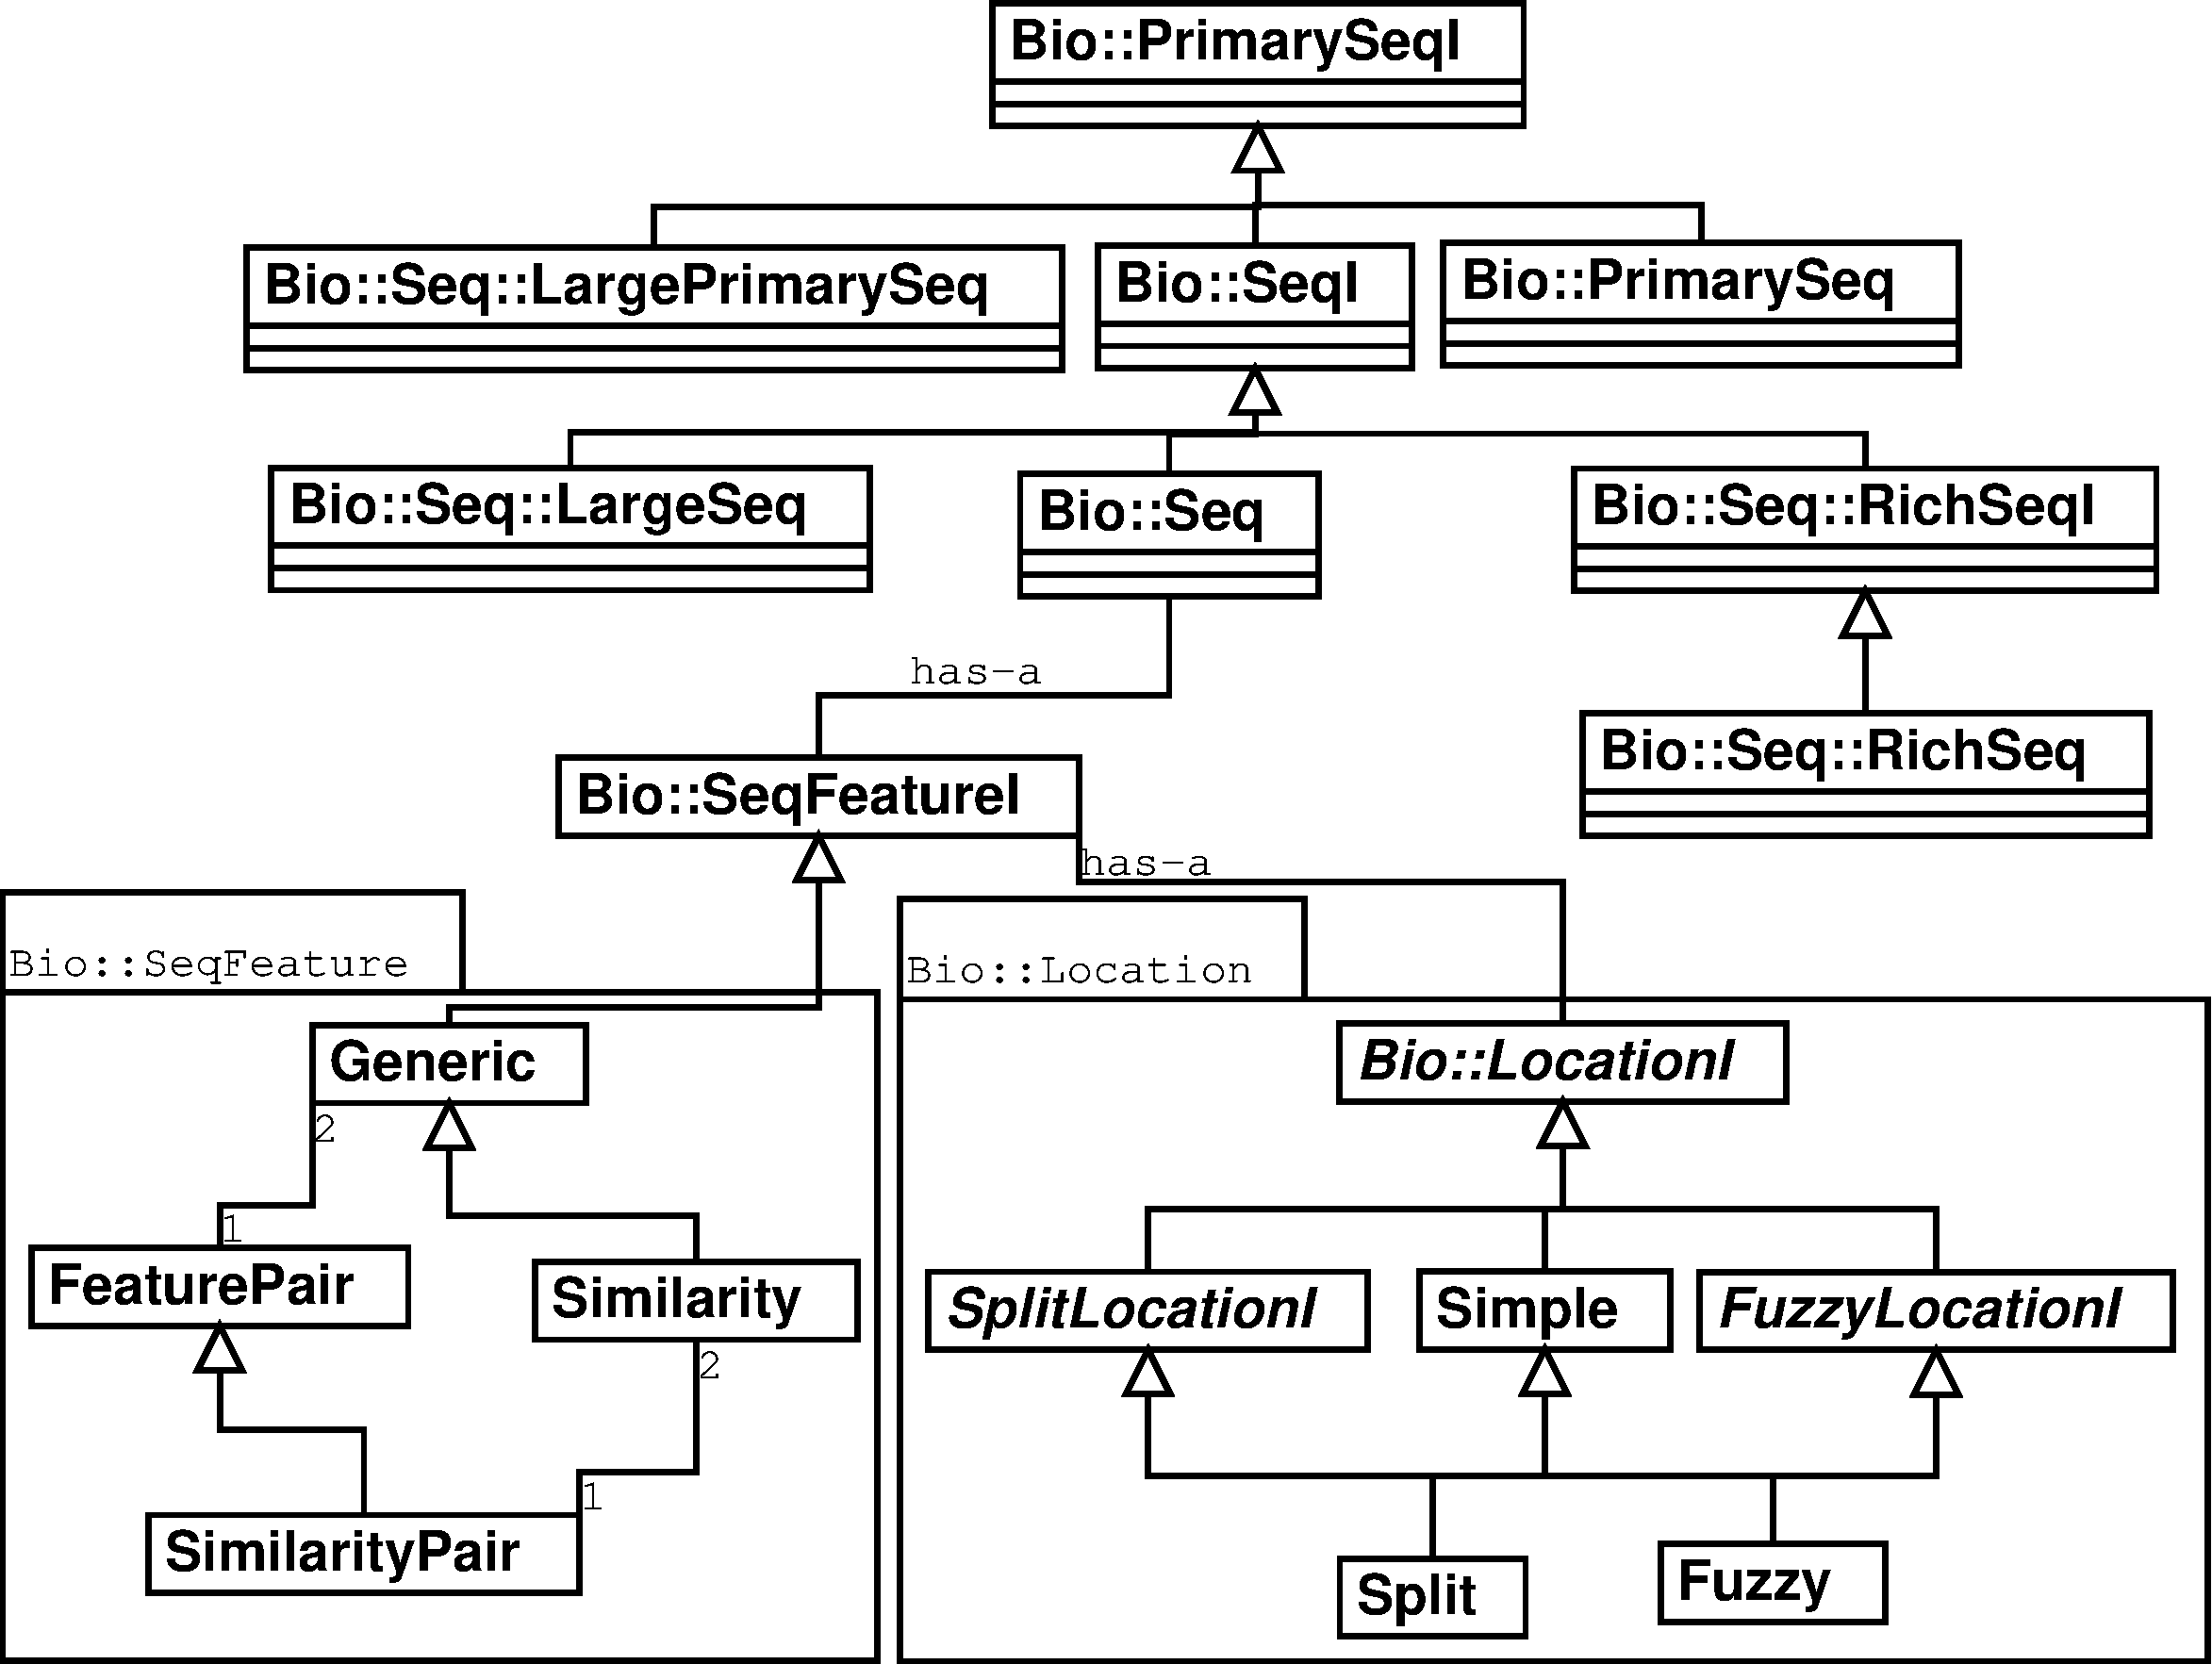
\epsfig{file=objectdiagram.pdf, width=8in}}
%\end{figure}

\newpage

\rhead{Stajich\_Figure3}
\begin{verbatim}
use Bio::DB::EMBL;
use Bio::SeqIO;

my $db = new Bio::DB::EMBL();
my $seq = $db->get_Seq_by_acc("U14680");
my $seqout = new Bio::SeqIO( -format => "genbank");
if (defined $seq) { # in case DB doesn't return anything
   $seqout->write_seq($seq);
}
\end{verbatim}
% $

\newpage

\rhead{Stajich\_Figure4}
\begin{verbatim}
use Bio::SearchIO;
# Let's parse a BLAST report 
my $search = new Bio::SearchIO( -format => 'blast',
                                -file   => 'report.bls');
my @HitsToSave = ();
my $cutoff_Evalue = 0.001; # max e-value is 0.001
my $cutoff_Len    = 120;   # min length of 120 residues
# iterate over each query sequence
while(my $result   = $search->next_result) {
 # iterate over each hit on the query sequence
 while(my $hit = $result->next_hit) {
   # iterate over each HSP in a hit
   while( my $hsp  = $hit->next_hsp ) {
    if( $hsp->evalue < $cutoff_Evalue && 
        $hsp->length('total') >= $cutoff_Len ) { 
        push @HitsToSave, $hit;
        last;
      } 
    }
  }
}
# process hits that met criteria
print "Hits:\n";
foreach my $hit ( @HitsToSave ) {
  print $hit->name, "\n";	
}

\end{verbatim}

\end{document}
